%%%%%%%%%%%%%%%%%%%%%%%%%%%%%%%%%%%%%%%%%%%%%%%%%%%%%%%%%%%%%%%%%%%%%%
% How to use writeLaTeX: 
%
% You edit the source code here on the left, and the preview on the
% right shows you the result within a few seconds.
%
% Bookmark this page and share the URL with your co-authors. They can
% edit at the same time!
%
% You can upload figures, bibliographies, custom classes and
% styles using the files menu.
%
%%%%%%%%%%%%%%%%%%%%%%%%%%%%%%%%%%%%%%%%%%%%%%%%%%%%%%%%%%%%%%%%%%%%%%

\documentclass[12pt]{article}

\usepackage{sbc-template}

\usepackage{graphicx,url}
\usepackage{multirow}
\usepackage{tabularx}
\usepackage[brazil]{babel}   
\usepackage[utf8]{inputenc}  
\usepackage{float}
\usepackage{xcolor}
\usepackage{url}
\usepackage{hyperref}
\usepackage{tabularx}
\usepackage{amsmath}
\usepackage{comment}
\usepackage{booktabs}
\usepackage[table]{xcolor}
\usepackage{makecell}

\newcommand{\dlr}[1]{\textcolor{red}{[DLR: #1]}}

     
\sloppy

% \title{AraraFin: Uma Solução Baseada em Large Language Models para Análise de Sentimentos Sensível aos Subdomínios do Mercado Financeiro Brasileiro}

\title{AraraFin: A Large Language Model-Based Solution for Domain-Sensitive Sentiment Analysis in the Brazilian Financial Market}

\author{Anônimo\inst{1}}

\address{Instituição Anônima
  \email{E-mail Anônimo}
}

 %\author{
 %  Vinícius L. Valente\inst{1},
 %  Romulo L. Bezerra\inst{1},
 %  Rafael G. M. dos Santos\inst{2},\\
 %  Denis Rosário\inst{1},
 %  Iago Medeiros\inst{1}
 %}
 %    \vspace{-3em}
 %\address{
 %  Universidade Federal do Pará (UFPA)
 %  \nextinstitute
 %  T2 Educação
 %  \email{\{vinicius.valente, romulo.bezerra\}@tucurui.ufpa.br}
 %  \email{rafaelgarcia1303@gmail.com}
 %  \email{\{denis, iagomedeiros\}@ufpa.br} 
%}


\begin{document} 

\maketitle

\begin{abstract}
This paper presents \textit{AraraFin}, a web-based sentiment analysis solution designed to support decision-making in the Brazilian financial market. The approach performs domain-aware sentiment classification through specialized prompts for Fixed Income, FIIs (Brazilian REITs) and Stocks. For the experimental evaluation, a manually annotated news dataset was constructed. The results indicate that \textit{AraraFin} outperformed \textit{FinBERT-PT-BR} across all analyzed modalities, achieving accuracy gains exceeding 100\% for FIIs and Fixed Income, and 12\% for Stocks. In addition, the analysis shows that smaller models can reach competitive performance when combined with appropriate prompts, with a better trade-off between cost and classification quality.
\end{abstract}

% \begin{resumo}
% Este trabalho apresenta \textit{AraraFin}, uma solução web de análise de sentimentos voltada ao apoio à tomada de decisão no mercado financeiro brasileiro. A proposta realiza a classificação de sentimentos de forma sensível ao domínio, por meio de \textit{prompts} especializados para Renda Fixa, Fundo de Investimentos Imobiliários (FIIs) e Ações. Para a avaliação experimental, foi construído um \textit{dataset} de notícias anotado manualmente. Os resultados indicam que a \textit{AraraFin} obteve resultados superiores aos de \textit{FinBERT-PT-BR} em todas as modalidades analisadas, com ganhos de acurácia superiores a 100\% em FIIs e Renda Fixa, e de 12\% em Ações. Além disso, a análise evidencia que modelos menores podem alcançar desempenho competitivo quando combinados a \textit{prompts} adequados, com melhor relação entre custo e qualidade de classificações.
% \end{resumo}


\section{Introdução}

A era da informação, intensificada pela expansão da Internet, gerou um volume massivo de dados não estruturados, muitos dos quais contêm informações valiosas capazes de sustentar decisões estratégicas em diversos setores. No mercado financeiro, a análise desses dados por meio de técnicas computacionais tem demonstrado desempenho superior na previsão de variações nos preços de ativos quando comparada às abordagens puramente estatísticas \cite{darwish2025stockforecasting}.

Diante deste contexto da mineração de dados, destaca-se a Análise de Sentimentos, um subcampo do Processamento de Linguagem Natural (PLN) que busca identificar, classificar e interpretar emoções ou opiniões expressas em textos. Por meio da Classificação Léxica, Modelos de Linguagem e Aprendizado de Máquina, a análise de sentimentos é um processo que analisa as palavras e o contexto para determinar a polaridade (positiva, negativa ou neutra), bem como quantifica opiniões subjetivas em dados mensuráveis \cite{caseli2024processamento}. 

Textos financeiros, como notícias, relatórios de analistas e publicações em redes sociais, possuem uma característica singular: capturam expectativas e reações emocionais dos agentes de mercado antes que essas percepções se reflitam nos preços dos ativos. Isso posiciona a análise de sentimentos não apenas como técnica de mineração de texto, mas como componente preditivo em sistemas de apoio à decisão de investimento, aplicável a ações, títulos de renda fixa e fundos imobiliários \cite{darwish2025stockforecasting}. Contudo, essa aplicabilidade traz consigo desafios específicos do domínio financeiro.

Conforme evidenciado por \cite{mahendran2025comparative}, os modelos de linguagem requerem adaptações substanciais para diferentes mercados regionais e idiomas, uma vez que a terminologia financeira assume significados específicos e nuances interpretativas que variam conforme o contexto cultural e econômico. Tecnicamente, essas adaptações podem ser realizadas por meio de \textit{fine-tuning} de modelos como o BERT, que requer datasets rotulados e treinamento computacionalmente custoso, ou através de \textit{prompt engineering} em Grandes Modelos de Linguagem (do inglês \textit{Large Language Models} - LLMs) disponibilizados via API por empresas como a OpenAI e a Anthropic, que dispensam re-treinamento mas implicam custos recorrentes por requisição.

No panorama brasileiro, esta questão se torna ainda mais relevante, pois existe uma notável escassez de ferramentas específicas tanto para o setor financeiro quanto para o português brasileiro, como apontado por \cite{santos2023finbert}. Este fator limita significativamente a eficácia das análises de sentimento para investidores e instituições que atuam no mercado nacional.

Diante desse cenário, este artigo apresenta a \textit{AraraFin}, uma ferramenta baseada em LLM para análise de sentimentos que atua no apoio à decisão para investidores brasileiros. A aplicação busca preencher uma lacuna relevante no domínio financeiro em português brasileiro, com adaptação da análise de sentimentos aos contextos específicos das três modalidades de investimento mais populares no país: Renda Fixa, Fundos de Investimento Imobiliário (FIIs) e Ações \cite{anbima2024}. Além disso, o trabalho avalia a escolha de um LLM a ser integrado, com base no desempenho e na relação custo-benefício. Os resultados indicam que a \textit{AraraFin} obteve desempenho superior ao da ferramenta de referência em todas as modalidades avaliadas, com ganhos de acurácia, e que o \textit{Sabiazinho 3} oferece a melhor relação custo-benefício entre os modelos avaliados.

O artigo está organizado da seguinte forma. A Seção 2 apresenta os trabalhos relacionados. A Seção 3 descreve a metodologia, a Seção 4 apresenta a \textit{AraraFin} e a Seção 5 discute os resultados. Por fim, a Seção 6 apresenta as conclusões.

\section{Trabalhos Relacionados} \label{sec:firstpage}

O desenvolvimento do \textit{FinBERT-PT-BR} por \cite{santos2023finbert} representou um marco significativo para a análise de texto no mercado financeiro brasileiro. Este modelo, treinado com um extenso \textit{corpus} de dados financeiros nacionais, habilitou aplicações diversas como Análise de Sentimentos, interpretação de relatórios corporativos e classificação de documentos financeiros. A contribuição foi relevante, em virtude de que, até então, a alternativa mais popular se limitava ao \textit{FinBERT} \cite{yang2020finbert}, desenvolvido para o mercado americano, na língua inglesa. Apesar disso, o \textit{FinBERT-PT-BR} foi idealizado para atender demandas gerais do domínio financeiro, e não especificidades contextuais que diferentes modalidades de investimento requerem.

Na revisão sistemática conduzida por \cite{jim2024recent} sobre os avanços e desafios da Análise de Sentimentos baseada em PLN, foram identificadas limitações críticas nas abordagens atuais. Segundo os autores, os modelos especializados como o \textit{FinBERT-PT-BR}, embora eficazes, demandam custos computacionais elevados e grandes volumes de dados rotulados, além de operarem como ``caixas-pretas"\,   
sem transparência nos processos decisórios. Além disso, os pesquisadores enfatizam a necessidade de aprimoramentos em dois aspectos fundamentais: compreensão contextual e adaptação de domínio, questões também destacadas por \cite{mahendran2025comparative}.

Nesse contexto, \cite{beltramini2024analise} compararam a eficácia do \textit{FinBERT-PT-BR} e \textit{GPT-3.5 Turbo} na análise de sentimentos sobre o IBOVESPA em redes sociais. Os resultados demonstraram a superioridade do \textit{GPT-3.5 Turbo} em acurácia e adequação contextual, apesar de ser uma solução paga em contraste com o modelo de código aberto. Vale ressaltar que o estudo utilizou uma versão legada do \textit{GPT-3.5} (2021), e se limitou a notícias relacionadas ao índice IBOVESPA, não explorando as especificidades de diferentes tipos de investimento. Além disso, modelos mais recentes, como o \textit{GPT-5.1} \cite{openai-docs}, já foram lançados e podem apresentar resultados melhores.

Embora a eficácia dos modelos da \textit{OpenAI} seja amplamente reconhecida, questões sobre seu desempenho em língua portuguesa motivaram investigações específicas. O estudo de \cite{de2024explorando} realizou uma análise comparativa entre os modelos \textit{GPT-4}, \textit{GPT-3.5 Turbo} e Sabiá 2, este último desenvolvido exclusivamente para o português e disponibilizado por meio da Maritaca \textit{AI}. Os resultados confirmaram que o \textit{GPT-4} apresentou melhor desempenho na classificação de polaridades dos textos. Entretanto, modelos mais avançados da Maritaca \textit{AI} já foram lançados, como o Sabiá 3.1 \cite{maritaca_modelos}, o que motiva a necessidade de reavaliação comparativa com as versões mais recentes, principalmente neste contexto do mercado financeiro brasileiro.

A Tabela~\ref{tab:trabalhos_relacionados} resume os trabalhos relacionados e suas limitações. Diante deste panorama, torna-se relevante investigar qual provedor de \textit{LLM} oferece a melhor relação entre desempenho e custos, de modo a apoiar a tomada de decisão dos investidores. Nesse contexto, este artigo irá apresentar uma análise comparativa do desempenho dos modelos \textit{GPT-5.1}, \textit{GPT-5-mini} e \textit{GPT-4o} (\textit{OpenAI}), bem como Sabiá 3.1 e Sabiazinho 3 (Maritaca \textit{AI}), na classificação de sentimentos de notícias do mercado financeiro quanto ao seu impacto em FIIs, Ações e Renda Fixa. Diferentemente dos estudos anteriores, esta investigação concentra-se em versões mais recentes dos modelos, amplia o escopo de análise para diferentes modalidades de investimento e considera o \textit{trade-off} entre desempenho e custos de uso. Por fim, os resultados obtidos serão comparados com a ferramenta \textit{FinBERT-PT-BR}, com o objetivo de validar a eficácia da aplicação proposta.

\begin{comment}
\begin{table}[h]
\centering
\caption{Resumo comparativo dos trabalhos relacionados}
\label{tab:trabalhos_relacionados}
\begin{tabularx}{\textwidth}{|X|X|X|}
\hline
\textbf{Trabalho} & \textbf{Contribuição} & \textbf{Limitações} \\
\hline
\cite{santos2023finbert} & \textit{FinBERT-PT-BR}: Ferramenta de análise de sentimentos em português & Não trata especificidades de FIIs, Ações e Renda Fixa \\
\hline
\cite{jim2024recent} & Identifica desafios e avanços da PLN no mercado financeiro & Alto custo computacional, grandes volumes de dados rotulados, ``caixa-preta'' \\
\hline
\cite{beltramini2024analise} & Compara \textit{FinBERT-PT-BR} e \textit{GPT-3.5 Turbo} em notícias do IBOVESPA & Limitado a notícias do IBOVESPA; versão legada do GPT-3.5 \\
\hline
\cite{de2024explorando} & Avaliação de GPT-4, GPT-3.5 e Sabiá 2 em português & Não inclui modelos mais recentes da Maritaca (\textit{Sabiá 3.1}, \textit{Sabiazinho 3}) \\
\hline
\end{tabularx}
\end{table}
\end{comment}


\begin{table}[!htb]
\centering
\caption{Resumo comparativo dos trabalhos relacionados}
\label{tab:trabalhos_relacionados}
\resizebox{\textwidth}{!}{%
\begin{tabular}{@{}lcc@{}}
\toprule
\textbf{Trabalho} & \textbf{Contribuição} & \textbf{Limitações} \\ \midrule
\rowcolor{gray!30}\cite{santos2023finbert} & 
\textit{FinBERT-PT-BR}: Ferramenta de análise de sentimentos em português & 
Não trata especificidades de FIIs, Ações e Renda Fixa \\

\cite{jim2024recent} & 
Identifica desafios e avanços da PLN no mercado financeiro & 
Alto custo computacional, grandes volumes de dados rotulados, ``caixa-preta'' \\

\rowcolor{gray!30}\cite{beltramini2024analise} & 
Compara \textit{FinBERT-PT-BR} e \textit{GPT-3.5 Turbo} em notícias do IBOVESPA & 
Limitado a notícias do IBOVESPA; versão legada do GPT-3.5 \\

\cite{de2024explorando} & 
Avaliação de GPT-4, GPT-3.5 e Sabiá 2 em português & 
Não inclui modelos mais recentes da Maritaca (\textit{Sabiá 3.1}, \textit{Sabiazinho 3}) \\

\bottomrule
\end{tabular}%
}
\end{table}





\section{\textit{Metodologia}}

Esta seção apresenta a metodologia adotada para a avaliação dos LLMs no contexto da \textit{AraraFin}. São descritos os procedimentos utilizados para a construção do \textit{dataset} de referência, a estratégia de classificação e a organização da \textit{pipeline} experimental.

\subsection{Construção do \textit{Dataset} de Referência}


% Foi construído um \textit{dataset} \footnote{\textbf{\textit{Dataset} de referência:} disponível em \href{https://github.com/vinelouzada/ararafin-research/blob/main/analise_sentimentos_textos_financeiros_gabarito.csv}
% {\textcolor{blue}{repositório público no GitHub}}.} próprio, uma vez que não foram encontrados conjuntos de dados públicos e atualizados referentes aos anos de 2025 e 2026 que contemplassem simultaneamente as três modalidades de investimento analisadas neste artigo. A Figura~\ref{fig:resumo-dataset} apresenta o processo de construção do \textit{dataset} de referência. 

Foi construído um \textit{dataset}\footnote{\textbf{\textit{Dataset} de referência:} disponível em \href{https://github.com/pesquisador-anonimo/ararafin-research/blob/master/analise_sentimentos_textos_financeiros_gabarito.csv}{\textcolor{blue}{repositório anônimo no GitHub}} (para avaliação cega)} próprio, uma vez que não foram encontrados conjuntos de dados públicos e atualizados referentes aos anos de 2025 e 2026 que contemplassem simultaneamente as três modalidades de investimento analisadas neste artigo. A Figura~\ref{fig:resumo-dataset} apresenta o processo de construção do \textit{dataset} de referência.

%Este conjunto% \footnote{\textbf{\textit{Dataset} de referência:} disponível em \href{https://github.com/vinelouzada/ararafin-research/blob/main/analise_sentimentos_textos_financeiros_gabarito.csv}
%{\textcolor{blue}{repositório público no GitHub}}.} é utilizado na avaliação dos LLMs. A Seção~\ref{sec:selecao-llms} apresenta os modelos considerados na análise.

\begin{figure}[ht]
\centering
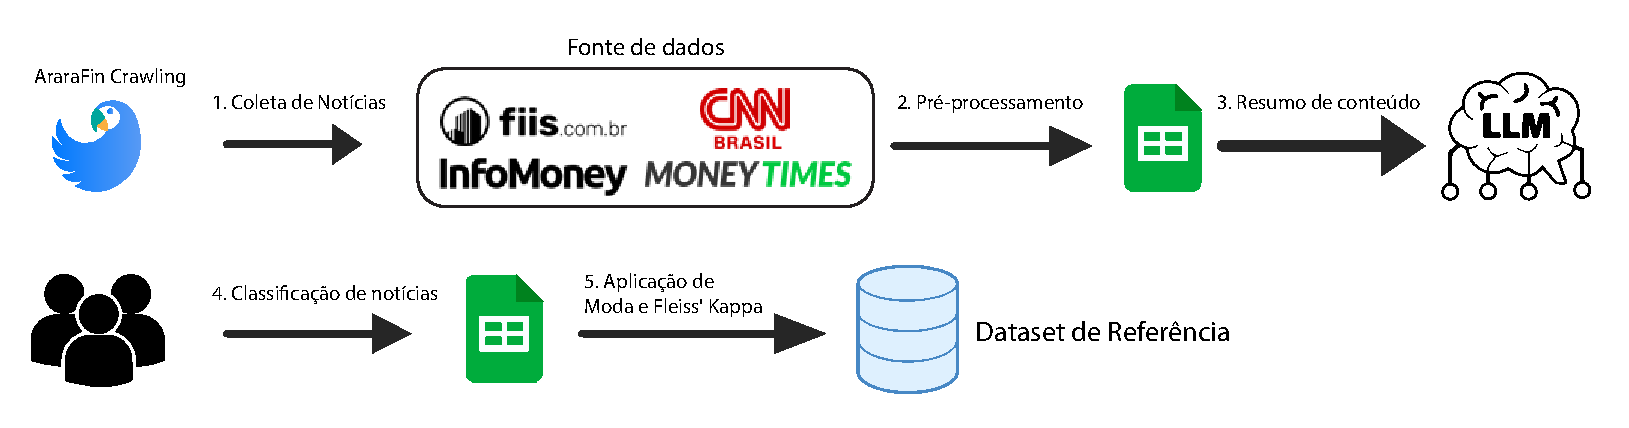
\includegraphics[width=.8\textwidth]{fluxo-dataset.pdf}
\caption{Fluxo resumido do processo de construção do dataset de referência.}
\label{fig:resumo-dataset}
\end{figure}


% A coleta dos dados foi realizada por meio de um processo automatizado de \textit{web scraping}\footnote{\textit{AraraFin Crawling}, desenvolvido para a coleta automatizada de notícias financeiras, disponível em \href{https://github.com/vinelouzada/ararafin-crawling}{\textcolor{blue}{repositório público no GitHub}}.}, aplicado a quatro veículos especializados em economia e mercado financeiro: \textit{InfoMoney}, \textit{FIIs Notícias}, \textit{MoneyTimes} e \textit{CNN Brasil}. O procedimento foi executado diariamente ao longo de um período de vinte dias. Para cada notícia coletada, foram armazenados o título, o conteúdo textual, a data de publicação, a data de coleta, a fonte e a respectiva URL, de modo a garantir rastreabilidade e organização do conjunto de dados. Inicialmente, foram obtidos 780 textos. Em seguida, aplicou-se uma etapa de pré-processamento para remoção de duplicatas e registros incompletos. Após essa etapa de limpeza, o conjunto final passou a conter 628 textos, aos quais foi acrescentado um campo adicional contendo um resumo do conteúdo original, elaborado com o auxílio de um LLM. Esse procedimento visa facilitar o processo de classificação manual e reduzir o custo com \textit{tokens}\footnote{Em LLMs, \textit{tokens} representam unidades mínimas de texto, sendo o custo proporcional à quantidade processada.} associado às etapas posteriores de avaliação.


A coleta dos dados foi realizada por meio de um processo automatizado de \textit{web scraping}\footnote{\textit{AraraFin Crawling}, desenvolvido para a coleta automatizada de notícias financeiras, disponível em \href{https://github.com/pesquisador-anonimo/ararafin-crawling}{\textcolor{blue}{repositório anônimo no GitHub}} (para avaliação cega)}, aplicado a quatro veículos especializados em economia e mercado financeiro: \textit{InfoMoney}, \textit{FIIs Notícias}, \textit{MoneyTimes} e \textit{CNN Brasil}. O procedimento foi executado diariamente ao longo de um período de 24 dias, entre 12 de agosto e 05 de setembro de 2025. Para 
cada notícia coletada, foram armazenados o título, o conteúdo textual, a data de publicação, a data de coleta, a fonte e a respectiva URL, de modo a garantir rastreabilidade e organização 
do conjunto de dados. Inicialmente, foram obtidos 780 textos. Em seguida, aplicou-se uma etapa de pré-processamento automatizada por meio de um \textit{script} em \textit{Python}, responsável pela remoção de duplicatas e de registros com corpo textual vazio. Após essa etapa de limpeza, o conjunto final passou a conter 628 textos, aos quais foi acrescentado um campo adicional contendo um resumo do 
conteúdo original, elaborado com o auxílio de um LLM. Tanto a classificação manual realizada pelos avaliadores quanto as classificações automatizadas executadas pelos modelos
nas etapas experimentais utilizaram esses resumos como entrada, o que contribui para a redução do custo com \textit{tokens}\footnote{\textit{tokens} representam unidades mínimas 
de texto, sendo o custo proporcional à quantidade processada.} e para a padronização do processo de avaliação.

A composição do dataset final apresenta a seguinte distribuição por fonte: \textbf{MoneyTimes} (299 notícias, 47,6\%), \textbf{InfoMoney} (141 notícias, 22,5\%), \textbf{FIIs Notícias} (122 notícias, 19,4\%) e \textbf{CNN Brasil} (66 notícias, 10,5\%). A classificação do conjunto de dados foi realizada manualmente por quatro avaliadores, dos quais três são engenheiros e um profissional credenciado atuante no mercado financeiro. Cada avaliador realizou a classificação de forma independente e atribuiu a cada notícia uma categoria de impacto (positivo, negativo ou neutro) em relação a cada uma das modalidades de investimento analisadas. Para a definição do rótulo final, adotou-se o critério da moda, no qual a classe mais frequentemente atribuída pelos avaliadores para cada texto e domínio foi considerada como rótulo definitivo. Nos casos em que houve empate entre as classificações, a anotação fornecida pelo especialista do mercado financeiro foi utilizada como critério de desempate. 
A escolha metodológica de incluir múltiplos avaliadores, ao invés de depender exclusivamente do especialista, justifica-se pela necessidade de mitigar possíveis vieses
individuais e reduzir o risco de erro sistemático, dado que mesmo profissionais experientes estão sujeitos a interpretações enviesadas em determinados contextos. Esse procedimento contribuiu para aumentar a consistência e a confiabilidade do conjunto de dados anotado.

Em relação à distribuição das classes de sentimento resultantes em cada domínio, observa-se que, para Renda Fixa, predominam classificações neutras (90,0\%), seguidas de positivas (6,1\%) e negativas (4,0\%). No domínio de FIIs, a distribuição é de 65,0\% neutras, 25,6\% positivas e 9,4\% negativas. Já no domínio de Ações, verifica-se maior equilíbrio entre as classes: 45,7\% neutras, 31,1\% positivas e 23,2\% negativas.

O desbalanceamento observado reflete características intrínsecas de cada modalidade. A predominância de neutras em Renda Fixa (90,0\%) é consistente com a menor volatilidade 
desse mercado, cujos ativos respondem principalmente a indicadores macroeconômicos estruturais como Selic e inflação, com divulgação predominantemente descritiva. Os FIIs apresentam distribuição 
intermediária (65,0\% neutras), característica de sua natureza híbrida entre renda fixa e variável. O maior equilíbrio em Ações (45,7\% neutras) decorre da alta sensibilidade desse mercado a eventos
corporativos e mudanças nas expectativas econômicas. A opção por preservar a distribuição natural garante avaliação em condições representativas do cenário real, o que aumenta a validade ecológica da ferramenta.

Como forma de avaliar a consistência desse processo, a concordância entre os avaliadores foi mensurada por meio do coeficiente de Fleiss (\textit{Fleiss' Kappa}), apropriado para cenários com mais de dois anotadores e categorias nominais.  O coeficiente de Fleiss é definido conforme a Equação~\ref{eq:fleiss}, que expressa a concordância observada entre os avaliadores, ajustada pela concordância esperada ao acaso.

\begin{equation}
\kappa = \frac{\bar{P} - \bar{P_e}}{1 - \bar{P_e}}
\label{eq:fleiss}
\end{equation}

% Onde $\bar{P}$ é a concordância média observada, calculada como a média das proporções de concordância entre todos os avaliadores para cada item, e $\bar{P_e}$ é a concordância esperada ao acaso, obtida a partir das proporções marginais de cada categoria sobre todos os avaliadores. O valor de $\kappa$ varia de $-1$ a $1$, sendo $\kappa = 1$ indicativo de concordância perfeita, $\kappa = 0$ de concordância equivalente à esperada ao acaso, e valores negativos sinalizam discordância sistemática. Os valores obtidos\footnote{\textbf{Análise e geração do \textit{dataset}:} disponível em 
% \href{https://github.com/vinelouzada/ararafin-research/blob/main/Consolida\%C3\%A7\%C3\%A3o\_do\_Dataset\_de\_Refer\%C3\%AAncia\_not\%C3\%ADcias\_rotuladas\_do\_mercado\_financeiro\_brasileiro.ipynb}
% {\textcolor{blue}{repositório público no GitHub}}.}
%  indicaram concordância moderada para FIIs ($\kappa = 0{,}56$) e Ações ($\kappa = 0{,}57$), e concordância razoável para Renda Fixa ($\kappa = 0{,}35$), que reflete a maior subjetividade envolvida na interpretação desse domínio.

Onde $\bar{P}$ é a concordância média observada e $\bar{P_e}$ é a concordância esperada ao acaso. O valor de $\kappa$ varia de $-1$ a $1$, 
sendo $\kappa = 1$ de concordância perfeita, $\kappa = 0$ 
equivalente ao acaso, e valores negativos 
sinalizam discordância sistemática. Os valores obtidos%
\footnote{\textbf{Análise e geração do \textit{dataset}:} disponível em
\href{https://github.com/pesquisador-anonimo/ararafin-research/blob/master/Consolida\%C3\%A7\%C3\%A3o\_do\_Dataset\_de\_Refer\%C3\%AAncia\_not\%C3\%ADcias\_rotuladas\_do\_mercado\_financeiro\_brasileiro.ipynb}
{\textcolor{blue}{repositório anônimo no GitHub}} (para avaliação cega)}
indicaram concordância moderada para FIIs ($\kappa = 0{,}56$) e 
Ações ($\kappa = 0{,}57$), e concordância razoável para Renda 
Fixa ($\kappa = 0{,}35$), que reflete a maior subjetividade 
envolvida na interpretação desse domínio.



Para complementar a analise do \textit{dataset}, foi calculada a correlação de Pearson entre os rótulos dos três domínios, codificados como $+1$, $0$ e $-1$, sobre os 628 textos anotados. A Figura~\ref{fig:pearson-heatmap} apresenta o \textit{heatmap} resultante. Os resultados indicam correlação negativa entre Renda Fixa e FIIs
($r = -0{,}29$, $p < 0{,}001$) e entre Renda Fixa e Ações
($r = -0{,}21$, $p < 0{,}001$), e correlação positiva entre FIIs e Ações
($r = +0{,}29$, $p < 0{,}001$).
Esse padrão é coerente com a dinâmica do mercado financeiro: elevações da taxa
Selic tendem a beneficiar a Renda Fixa e a prejudicar FIIs e Ações, enquanto
esses dois domínios compartilham sensibilidade semelhante a variáveis
macroeconômicas, como inflação e nível de atividade econômica.
Os achados reforçam a pertinência da estratégia de \textit{prompts} segmentados
por domínio adotada pela \textit{AraraFin}.
Ressalta-se que Renda Fixa concentra 90\% dos rótulos na classe neutra, o que
atenua naturalmente sua correlação com os demais domínios, sem comprometer a
significância estatística dos resultados.

\begin{figure}[h!]
    \centering
    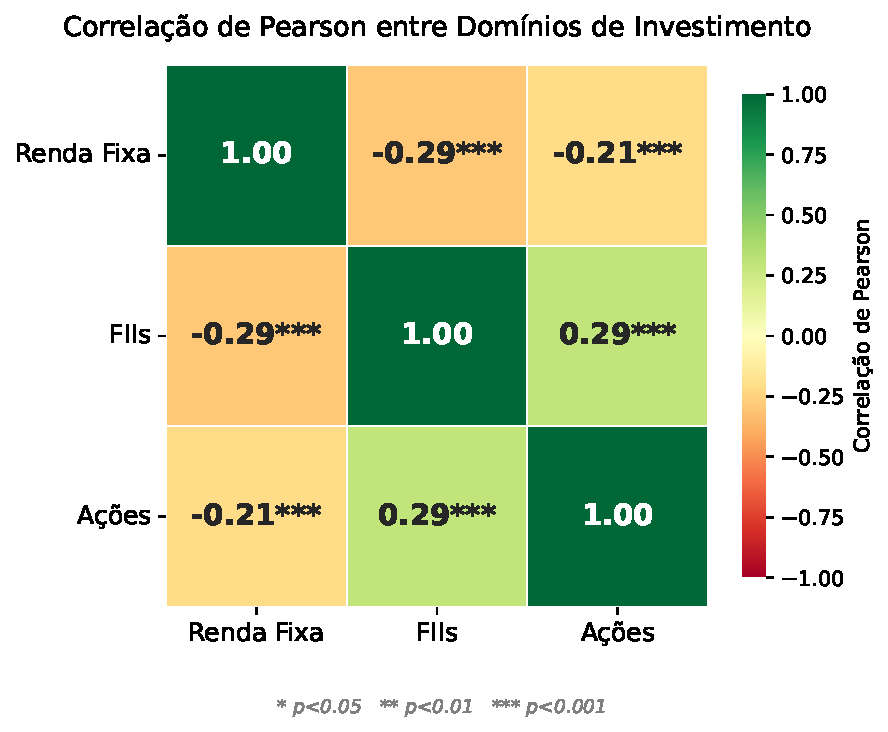
\includegraphics[width=0.5\textwidth]{pearson_heatmap.pdf}
    \caption{Correlação de Pearson entre os sentimentos atribuídos por domínio
    de investimento.}
    \label{fig:pearson-heatmap}
\end{figure}


\subsection{Seleção de LLMs}
\label{sec:selecao-llms}

A seleção dos \textit{LLMs} foi orientada por dois critérios centrais: (i) a capacidade de compreender e gerar respostas em português brasileiro; e (ii) a viabilidade econômica para uso em aplicações práticas. Com base nesses critérios, foram selecionados cinco modelos candidatos à integração no sistema: \textit{GPT-5.1}, \textit{GPT-5-mini}, \textit{GPT-4o}, Sabiá 3.1 e Sabiazinho 3. Especificamente, o \textbf{\textit{GPT-5.1}} é um dos modelos mais recentes da \textit{OpenAI}, voltado para tarefas de codificação e interação com agentes \cite{openai-docs}. O \textbf{\textit{GPT-5-mini}} é uma versão compacta do \textit{GPT-5}, indicada para tarefas bem definidas e instruções precisas, com menor custo operacional \cite{openai-docs}. O \textbf{\textit{GPT-4o}} é um modelo multimodal da \textit{OpenAI} flexível e caracterizado como o melhor modelo para a maioria das tarefas \cite{openai-docs}. O \textbf{Sabiá 3.1} é um modelo que apresenta desempenho notável em tarefas que exigem conhecimento recente \cite{maritaca_modelos}. Por fim, o \textbf{Sabiazinho 3} é um modelo projetado para aplicações que priorizam velocidade e custo \cite{maritaca_modelos}.

GPT-5.1 e GPT-5-mini são \textit{reasoning models} que executam múltiplas etapas de processamento lógico, enquanto GPT-4o é multimodal e de propósito geral \cite{openai-docs}. Sabiá 3.1 e Sabiazinho 3 são especializados em português brasileiro por \textit{continual learning} sem mecanismos nativos de raciocínio estendido \cite{maritaca_modelos}. A Tabela~\ref{tab:preco} apresenta a estrutura de precificação dos modelos avaliados, onde os valores originalmente expressos em dólar americano foram convertidos para real brasileiro, com base na taxa de câmbio de US\$~1{,}00 = R\$~5{,}16, conforme cotação vigente em 22/06/2026. Observa-se que o \textit{Sabiazinho 3} possui o menor custo por milhão de tokens, enquanto o \textit{GPT-4o} apresenta os maiores valores de entrada e saída entre os modelos analisados. %Desta forma, os modelos \textit{GPT-5.1}, \textit{GPT-5-mini}, \textit{GPT-4o}, Sabiá 3.1 e Sabiazinho 3 formam a base experimental deste estudo, sendo avaliados nas seções subsequentes.

\begin{comment}
\begin{table}[!htb]
\centering
\caption{Comparação de custo entre os modelos.}
\label{tab:preco}
\renewcommand{\arraystretch}{1.3}
\begin{tabularx}{\textwidth}{
|X|
>{\centering\arraybackslash}X|
>{\centering\arraybackslash}X|
>{\centering\arraybackslash}X|
>{\centering\arraybackslash}X|
>{\centering\arraybackslash}X|}
\hline
\textbf{Preço por milhão de tokens} 
& \textbf{\textit{GPT-5.1}} 
& \textbf{\textit{GPT-5-mini}} 
& \textbf{\textit{GPT-4o}} 
& \textbf{\textit{Sabiá 3.1}} 
& \textbf{\textit{Sabiazinho 3}} \\
\hline
Entrada 
& US\$ 1{,}25 \newline (R\$ 6{,}90) 
& US\$ 0{,}25 \newline (R\$ 1{,}38) 
& US\$ 2{,}50 \newline (R\$ 13{,}80) 
& R\$ 5{,}00 
& R\$ 1{,}00 \\
\hline
Saída 
& US\$ 10{,}00 \newline (R\$ 55{,}20) 
& US\$ 2{,}00 \newline (R\$ 11{,}04) 
& US\$ 10{,}00 \newline (R\$ 55{,}20) 
& R\$ 10{,}00 
& R\$ 3{,}00 \\
\hline
\end{tabularx}
\end{table}
\end{comment}

\begin{table}[!htb]
\centering
\caption{Comparação de custo entre os modelos.}
\label{tab:preco}
\renewcommand{\arraystretch}{1.3}
\resizebox{0.8\textwidth}{!}{%
\begin{tabular}{@{}lccccc@{}}
\toprule
\textbf{Preço por milhão de tokens} 
& \textbf{\textit{GPT-5.1}} 
& \textbf{\textit{GPT-5-mini}} 
& \textbf{\textit{GPT-4o}} 
& \textbf{\textit{Sabiá 3.1}} 
& \textbf{\textit{Sabiazinho 3}} \\
\midrule

\rowcolor{gray!30}Entrada 
& \shortstack{US\$ 1{,}25 \\ (R\$ 6{,}45)} 
& \shortstack{US\$ 0{,}25 \\ (R\$ 1{,}29)} 
& \shortstack{US\$ 2{,}50 \\ (R\$ 12{,}90)} 
& R\$ 5{,}00 
& R\$ 1{,}00 \\

Saída 
& \shortstack{US\$ 10{,}00 \\ (R\$ 51{,}58)} 
& \shortstack{US\$ 2{,}00 \\ (R\$ 10{,}32)} 
& \shortstack{US\$ 10{,}00 \\ (R\$ 51{,}58)} 
& R\$ 10{,}00 
& R\$ 3{,}00 \\

\bottomrule
\end{tabular}%
}
\end{table}


\subsection{\textit{Prompts} e Estratégias de Classificação}

% A \textit{AraraFin} utiliza uma estratégia de classificação 
% segmentada, na qual são definidos \textit{prompts}%
% \footnote{\textbf{\textit{Prompts} utilizados:} disponíveis em
% \href{https://github.com/vinelouzada/ararafin-research/blob/master/prompts.md}
% {\textcolor{blue}{repositório anônimo no GitHub}} (perfil ocultado 
% para avaliação cega).}.distintos para cada categoria de investimento. Essa escolha 
% decorre do fato de que diferentes domínios respondem de maneira 
% distinta a indicadores macroeconômicos e a notícias financeiras, 
% o que exige interpretações contextualizadas para a correta 
% identificação do sentimento associado.


A \textit{AraraFin} utiliza uma estratégia de classificação 
segmentada, na qual são definidos \textit{prompts}%
\footnote{\textbf{\textit{Prompts} utilizados:} disponíveis em
\href{https://github.com/pesquisador-anonimo/ararafin-research/blob/master/prompts.md}
{\textcolor{blue}{repositório anônimo no GitHub}} (perfil ocultado 
para avaliação cega).} distintos para cada categoria de investimento. Essa escolha 
decorre do fato de que diferentes domínios respondem de maneira 
distinta a indicadores macroeconômicos e a notícias financeiras, 
o que exige interpretações contextualizadas para a correta 
identificação do sentimento associado.

Para isso, adota-se a estratégia de \textit{role prompting}, na qual cada modelo é instruído a assumir o papel de um analista especializado em seu respectivo domínio e a considerar características próprias de cada segmento. Conforme descrito por \cite{b3_2025}, no caso das ações, devem ser considerados fatores relacionados ao desempenho corporativo e ao ambiente macroeconômico. Por exemplo, para os FIIs, deve-se considerar aspectos associados ao mercado imobiliário, enquanto, para a renda fixa, consideram-se elementos vinculados às taxas de juros, à inflação e ao risco de crédito. 

Como referência adicional, adota-se o estudo de \cite{andrade2022influencia}, que analisa a influência de variáveis macroeconômicas, como desemprego, inflação e taxa Selic, sobre o mercado acionário. Os princípios discutidos neste trabalho são considerados, de forma análoga, na atribuição de polaridade aos textos em cada domínio.
A Tabela~\ref{tab:exemplos-noticias} apresenta exemplos de trechos de notícias e suas polaridades atribuídas por domínio e ilustra como um mesmo evento pode ser interpretado de forma distinta, conforme o segmento de investimento.

\begin{comment}
\begin{table}[!htb]
\centering
\caption{Exemplos de notícias e polaridade por domínio de investimento}
\label{tab:exemplos-noticias}
\begin{tabular}{|p{5.5cm}|c|c|c|}
\hline
\textbf{Trecho da notícia} & \textbf{Ações} & \textbf{FIIs} & \textbf{Renda Fixa} \\
\hline
Selic elevada em 15\% pelo Banco Central & Negativo & Negativo & Positivo \\
\hline
Vacância do FII XPML11 aumentou para 10\% & Neutro & Negativo & Neutro \\
\hline
Magazine Luiza (MGLU3) cresceu acima do esperado no trimestre & Positivo & Neutro & Neutro \\
\hline
\end{tabular}
\end{table}    
\end{comment}

\begin{table}[!htb]
\centering
\caption{Exemplos de notícias e polaridade por domínio de investimento}
\label{tab:exemplos-noticias}
\resizebox{0.7\textwidth}{!}{%
\begin{tabular}{@{}lccc@{}}
\toprule
\textbf{Trecho da notícia} & \textbf{Ações} & \textbf{FIIs} & \textbf{Renda Fixa} \\
\midrule

\rowcolor{gray!30}
Selic elevada em 15\% pelo Banco Central & Negativo & Negativo & Positivo \\

Vacância do FII XPML11 aumentou para 10\% & Neutro & Negativo & Neutro \\

\rowcolor{gray!30}
Magazine Luiza (MGLU3) cresceu acima do esperado no trimestre & Positivo & Neutro & Neutro \\

\bottomrule
\end{tabular}%
}
\end{table}

Além disso, emprega-se a técnica de \textit{one-shot prompting}, na qual cada instrução contém um exemplo de classificação no formato \textit{JSON}, utilizado como referência estrutural para a resposta esperada \cite{boonstra2024prompt}. Essa prática contribui para padronizar as saídas e reduzir ambiguidades no processo de classificação. Por fim, as inferências são realizadas com temperatura igual a zero, o que assegura comportamento determinístico.


\subsection{\textit{Pipeline} Experimental}
\label{subsec:pipeline-experimental}

A Figura~\ref{fig:estrutura} apresenta uma visão geral do fluxo de processamento do sistema em um cenário de uso convencional, no qual sete passos são executados obrigatoriamente em cada requisição. No contexto experimental, o fluxo permanece o mesmo, sendo alterada apenas a origem da entrada, que passa a ser fornecida pelo \textit{script} mencionado.


\begin{figure}[ht]
    \centering
    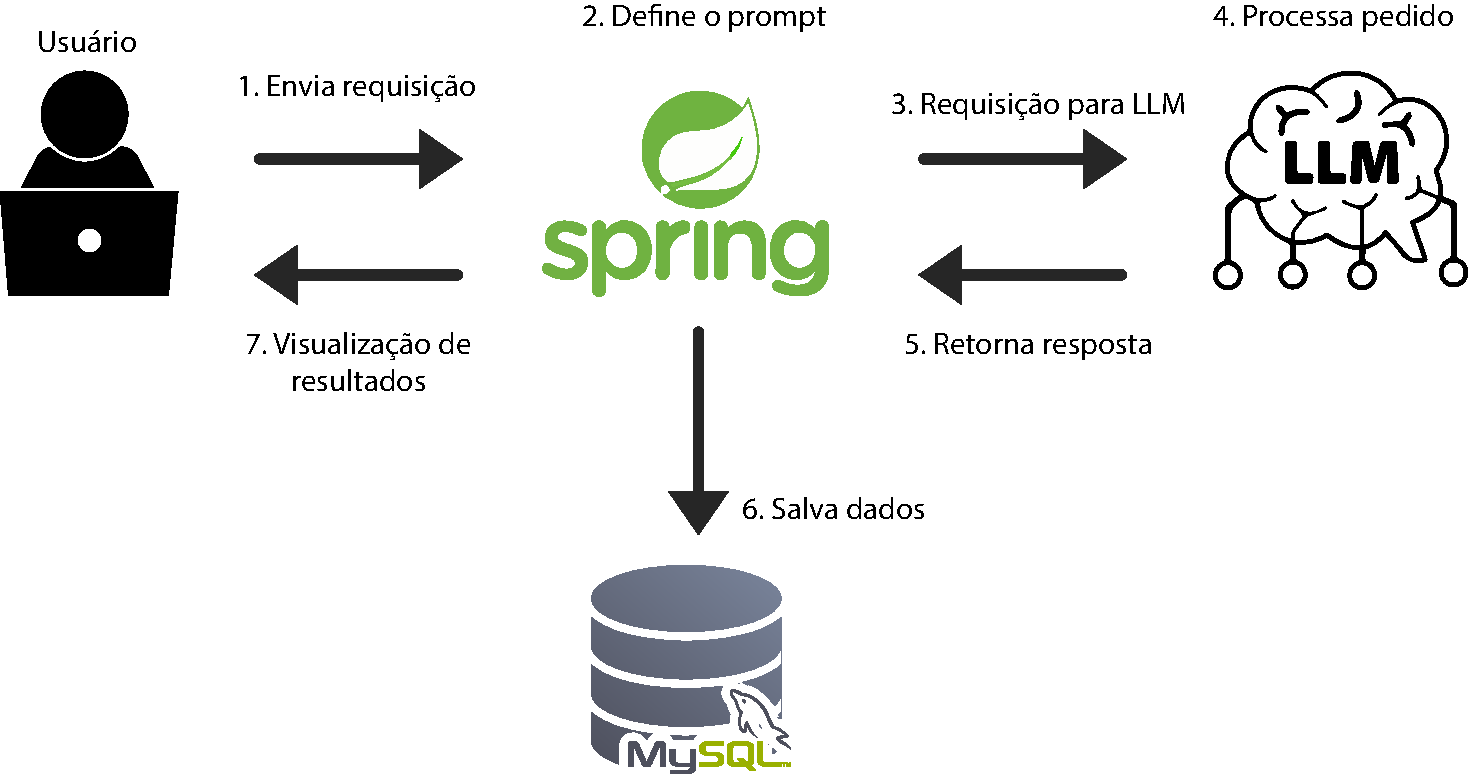
\includegraphics[width=.5\textwidth]{fluxo-ararafin.pdf}
    \caption{Fluxo de processamento da AraraFin.}
    \label{fig:estrutura}
\end{figure}

%O fluxo de processamento foi organizado em etapas sequenciais responsáveis por conduzir o texto de entrada até a geração da classificação. Em um cenário de uso, 
A AraraFin recebe um texto em linguagem natural fornecido pelo usuário, juntamente com a seleção do tipo de investimento (FIIs, Renda Fixa ou Ações) que o texto deve ser analisado. A partir dessas informações, o sistema seleciona automaticamente o \textit{prompt} correspondente ao domínio escolhido e realiza uma chamada síncrona a um modelo. O modelo processa a entrada e retorna uma resposta no formato \textit{JSON}, que contém a classe de sentimento prevista e sua respectiva justificativa. Essa resposta é armazenada em uma base de dados para fins de análise.

No contexto experimental, esse fluxo é executado de forma automatizada por meio de um \textit{script} em \textit{Python}, responsável por percorrer todo o \textit{dataset} de referência e submeter cada instância ao sistema. Como cada texto é classificado nos três domínios, são geradas 1.884 classificações a partir dos 628 textos do dataset. Esse procedimento foi repetido para cada modelo avaliado, o que permitiu uma comparação sistemática sob condições equivalentes de execução.

%A infraestrutura adotada para a realização dos experimentos foi local, pois reduz custos operacionais, minimiza atrasos de comunicação e garante maior controle sobre o ambiente de execução. Os experimentos foram conduzidos em um MacBook Air equipado com processador Apple M2 e 16~GB de memória RAM, configuração suficiente para a orquestração das chamadas aos modelos, o armazenamento dos resultados e a execução dos scripts de avaliação.



% \section{\textit{AraraFin}}

% Esta seção apresenta uma visão geral do desenvolvimento da \textit{AraraFin}, com foco nas motivações que orientaram a escolha das tecnologias, da arquitetura, bem como dos aspectos relacionados à identidade visual e à interface web.


% \subsection{Tecnologias Utilizadas}

% A solução foi desenvolvida segundo a arquitetura monolítica com \textit{Server-Side Rendering} (SSR). O back-end utilizou \textit{Spring Boot} 3.4.5 e \textit{Java} 21, enquanto o front-end empregou \textit{Thymeleaf} para a geração dinâmica de \textit{HTML}. A integração com \textit{LLMs} ocorreu por meio da biblioteca \textit{Spring AI}, o que possibilitou o uso de modelos da \textit{OpenAI} e da Maritaca AI. Os \textit{prompts}, textos analisados e respostas foram armazenados em um banco de dados \textit{MySQL}, e o código-fonte foi versionado no \textit{GitHub}.

% A aplicação foi implantada na \textit{Oracle Cloud}, em razão da disponibilidade de recursos gratuitos (\textit{Always Free}), que permitiram o uso da instância \textit{VM.Standard.E2.1.Micro} (1 OCPU e 1~GB de memória) e do serviço \textit{MySQL HeatWave} (50~GB de armazenamento, 1~ECPU e 8~GB de memória). A infraestrutura utilizou contêineres \textit{Docker}, \textit{NGINX} como \textit{proxy} reverso e \textit{Cloudflare} para gestão de DNS. As tecnologias foram selecionadas com base em critérios de custo-benefício e na experiência prévia dos autores.

% \subsection{Identidade Visual e Interface Web}

% A identidade visual da \textit{AraraFin} foi produzida para remeter ao contexto brasileiro; para isso, foi utilizada como elemento simbólico a arara-azul, bem como uma paleta de cores inspirada na bandeira nacional. O nome da solução resulta da combinação entre ``Arara'' e ``Financeiro''. A tipografia \textit{Sora}%
% \footnote{\textbf{Tipografia \textit{Sora}:} disponível em 
% \href{https://fonts.google.com/specimen/Sora}
% {\textcolor{blue}{Google Fonts}}.}
% foi escolhida por ser gratuita e amplamente compatível com navegadores. A interface%
% \footnote{\textbf{\textit{Screenshots} da solução:} disponíveis em
% \href{https://github.com/pesquisador-anonimo/ararafin-research/tree/master/ararafin-interfaces}
% {\textcolor{blue}{repositório anônimo no GitHub}} (perfil ocultado
% para avaliação).}
% adota padrões de \textit{design} comuns a plataformas como \textit{ChatGPT} e \textit{Gemini}, com o objetivo de reduzir a curva de aprendizado e favorecer a usabilidade. A Figura~\ref{fig:identidade} apresenta o resumo da identidade visual, e a Figura~\ref{fig:interface}, a interface.

% \begin{figure}[htbp]
% \centering

% \begin{minipage}{0.40\textwidth}
%     \centering
%     \includegraphics[width=\linewidth]{"ararafin-artigo copy.pdf"}
%     \caption{Identidade visual: \textit{AraraFin}.}
%     \label{fig:identidade}
% \end{minipage}
% \hfill
% \begin{minipage}{0.50\textwidth}
%     \centering
%     \includegraphics[width=\linewidth]{"interface da tela.png"}
%     \caption{Interface da \textit{AraraFin}.}
%     \label{fig:interface}
% \end{minipage}

% \end{figure}

\section{Resultados}

Nesta seção, são apresentados os resultados obtidos a partir da \textit{pipeline} experimental, com o objetivo de identificar o modelo adequado para integração à \textit{AraraFin}. Adicionalmente, realiza-se uma discussão crítica dos resultados, para destacar implicações, limitações e observações relevantes do experimento.

Foi adotada uma infraestrutura local para a realização dos experimentos, pois reduz custos operacionais, minimiza atrasos de comunicação e garante maior controle sobre o ambiente. Os experimentos foram conduzidos em um MacBook com processador Apple M2 e 16~GB de memória RAM, configuração suficiente para a orquestração das chamadas aos modelos, o armazenamento dos resultados e a execução dos scripts de avaliação.


Para avaliar o desempenho dos modelos, foram selecionadas métricas amplamente utilizadas em tarefas de classificação: Acurácia, Precisão e \textit{F1-score}.
A \textbf{Acurácia} mede a proporção de classificações corretas em relação ao total de amostras. A \textbf{Precisão} indica a proporção de instâncias corretamente classificadas como pertencentes a uma classe em relação ao total de instâncias atribuídas a essa classe.  Em cenários multiclasse, a métrica é obtida por meio da média aritmética das precisões individuais de cada classe. O \textbf{\textit{F1-Score}} corresponde à média harmônica entre a precisão e o recall, O \textbf{\textit{F1-Score}}, é útil em contextos com classes desbalanceadas, pois considera simultaneamente erros de falso positivo e falso negativo \cite{caseli2024processamento}. As métricas encontram-se normalizadas no intervalo $[0,1]$, no qual valores mais elevados indicam melhor desempenho.



\begin{comment}
\subsection{Métricas de Avaliação}

\begin{itemize}
  \item \textbf{Acurácia}: mede a proporção de classificações corretas em relação ao total de amostras, sendo definida por:
  \begin{equation}
    \text{Acurácia} = \frac{TP + TN}{TP + TN + FP + FN}
  \end{equation}
  onde $TP$ representa os verdadeiros positivos, $TN$ os verdadeiros negativos, $FP$ os falsos positivos e $FN$ os falsos negativos \cite{caseli2024processamento}.
  
  \item \textbf{Precisão}: indica a proporção de instâncias corretamente classificadas como pertencentes a uma classe em relação ao total de instâncias atribuídas a essa classe. Para uma dada classe, é calculada como:
  \begin{equation}
    \text{Precisão} = \frac{TP}{TP + FP}
  \end{equation}
  Em cenários multiclasse, a métrica é obtida por meio da média aritmética das precisões individuais de cada classe \cite{caseli2024processamento}.
  
  \item \textbf{\textit{F1-Score}}: corresponde à média harmônica entre a precisão e o recall, sendo definida por:
  \begin{equation}
    F1 = 2 \times \frac{\text{Precisão} \times \text{Recall}}{\text{Precisão} + \text{Recall}}
  \end{equation}
  Essa métrica é especialmente útil em contextos com classes desbalanceadas, pois considera simultaneamente erros de falso positivo e falso negativo \cite{caseli2024processamento}.
\end{itemize}

\end{comment}


\subsection{Análise Comparativa entre \textit{LLMs}}

A Tabela~\ref{tab:comparacao-gpt-sabia} apresenta os resultados da classificação de sentimentos por domínio de investimento, obtidos a partir da \textit{pipeline} experimental, o que permite a comparação direta entre os modelos avaliados. %De forma complementar, as Figuras~\ref{fig:acuracia-media}, \ref{fig:precisao-media} e \ref{fig:f1-media} sintetizam o desempenho médio dos modelos em relação aos tipos de investimento. 
A partir da Tabela~\ref{tab:comparacao-gpt-sabia}, observa-se que o \textit{GPT-4o} apresentou o melhor desempenho global, ao concentrar os maiores valores nas métricas avaliadas e na maioria dos domínios considerados. Esse resultado sugere maior robustez do modelo na identificação de sentimentos em diferentes contextos do mercado financeiro. Entretanto, essa superioridade não se manifestou de forma homogênea no domínio de FIIs, especificamente em termos de Acurácia, o \textit{Sabiazinho 3} apresentou desempenho superior ao do \textit{GPT-4o}, além de valores equivalentes nas métricas de Precisão e \textit{F1-score}. De modo semelhante, nos domínios de Renda Fixa e Ações, observou-se que os resultados dos dois modelos permaneceram muito próximos entre si. Esse comportamento indica que, embora o \textit{GPT-4o} seja um modelo de maior porte e capacidade geral, o \textit{Sabiazinho 3}, por ser um modelo menor, pode alcançar desempenho comparável em determinados contextos, especialmente quando associado a \textit{prompts} bem estruturados e adequados à tarefa.

\begin{comment}
\begin{table}[h!]
\centering
\caption{Comparação de desempenho dos modelos na classificação de sentimentos por domínio de investimento.}
\label{tab:comparacao-gpt-sabia}
\small
\begin{tabular}{|l|l|c|c|c|c|c|}
\hline
\textbf{Categoria} & \textbf{Métrica} 
& \textbf{Sabiá 3.1} 
& \textbf{Sabiazinho 3} 
& \textbf{GPT-4o} 
& \textbf{GPT-5-mini} 
& \textbf{GPT-5.1} \\
\hline

\multirow{3}{*}{FIIs} 
 & Acurácia   & 0.75 & \textbf{0.83} & 0.82 & 0.68 & 0.77 \\
 & Precisão   & 0.81 & \textbf{0.82} & \textbf{0.82} & 0.77 & 0.80 \\
 & \textit{F1-score} & 0.77 & \textbf{0.81} & \textbf{0.81} & 0.70 & 0.78 \\
\hline

\multirow{3}{*}{Renda Fixa} 
 & Acurácia   & 0.76 & 0.83 & \textbf{0.84} & 0.45 & 0.60 \\
 & Precisão   & \textbf{0.87} & 0.84 & \textbf{0.87} & \textbf{0.87} & \textbf{0.87} \\
 & \textit{F1-score} & 0.81 & 0.84 & \textbf{0.85} & 0.56 & 0.69 \\
\hline

\multirow{3}{*}{Ações} 
 & Acurácia   & 0.57 & 0.55 & \textbf{0.59} & 0.55 & 0.58 \\
 & Precisão   & 0.58 & 0.58 & \textbf{0.59} & 0.57 & \textbf{0.59} \\
 & \textit{F1-score} & 0.54 & 0.54 & \textbf{0.59} & 0.52 & 0.56 \\
\hline

\end{tabular}
\end{table}
\end{comment}


\begin{table}[!htb]
\centering
\caption{Comparação de desempenho dos modelos na classificação de sentimentos por domínio de investimento.}
\label{tab:comparacao-gpt-sabia}
\small
\resizebox{0.6\textwidth}{!}{%
\begin{tabular}{@{}llccccc@{}}
\toprule
\textbf{Categoria} & \textbf{Métrica} 
& \textbf{Sabiá 3.1} 
& \textbf{Sabiazinho 3} 
& \textbf{GPT-4o} 
& \textbf{GPT-5-mini} 
& \textbf{GPT-5.1} \\
\midrule

\multirow{3}{*}{FIIs} 
 & Acurácia   & 0.75 & \textbf{0.83} & 0.82 & 0.68 & 0.77 \\
 & Precisão   & 0.81 & \textbf{0.82} & \textbf{0.82} & 0.77 & 0.80 \\
 & \textit{F1-score} & 0.77 & \textbf{0.81} & \textbf{0.81} & 0.70 & 0.78 \\
\midrule

\multirow{3}{*}{Renda Fixa} 
 & Acurácia   & 0.76 & 0.83 & \textbf{0.84} & 0.45 & 0.60 \\
 & Precisão   & \textbf{0.87} & 0.84 & \textbf{0.87} & \textbf{0.87} & \textbf{0.87} \\
 & \textit{F1-score} & 0.81 & 0.84 & \textbf{0.85} & 0.56 & 0.69 \\
\midrule

\multirow{3}{*}{Ações} 
 & Acurácia   & 0.57 & 0.55 & \textbf{0.59} & 0.55 & 0.58 \\
 & Precisão   & 0.58 & 0.58 & \textbf{0.59} & 0.57 & \textbf{0.59} \\
 & \textit{F1-score} & 0.54 & 0.54 & \textbf{0.59} & 0.52 & 0.56 \\
\bottomrule

\end{tabular}%
}
\end{table}

\begin{comment}

\begin{figure}[h!]
    \centering
    
    % Primeira linha (2 figuras)
    \begin{minipage}{0.49\textwidth}
        \centering
        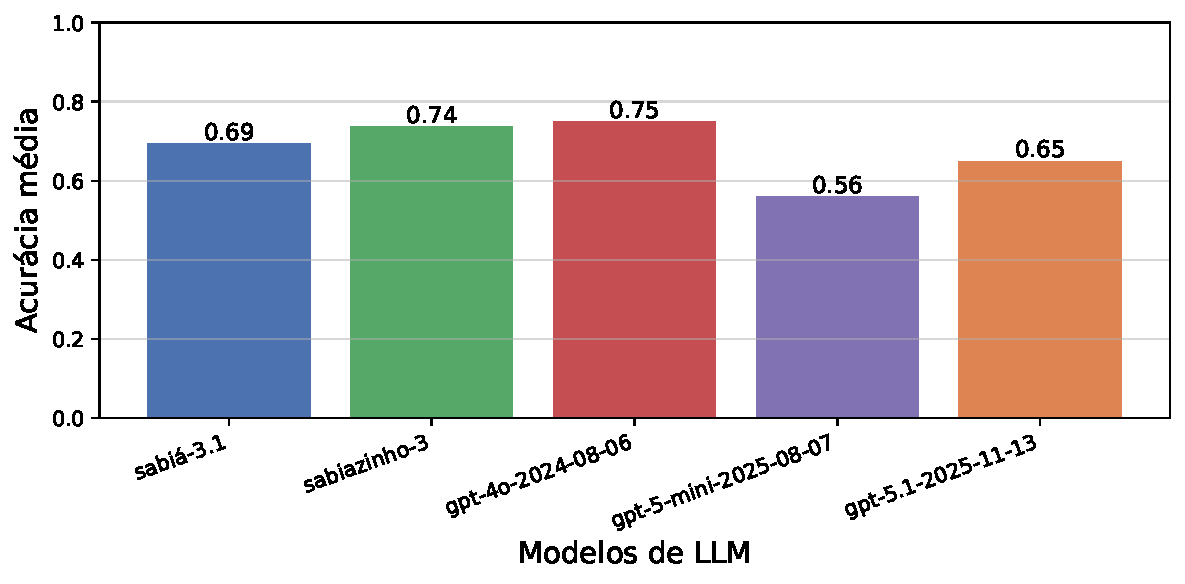
\includegraphics[width=\linewidth]{acuaria_media.pdf}
        \caption{Acurácia média dos modelos de LLM}
        \label{fig:acuracia-media}
    \end{minipage}
    \hfill
    \begin{minipage}{0.49\textwidth}
        \centering
        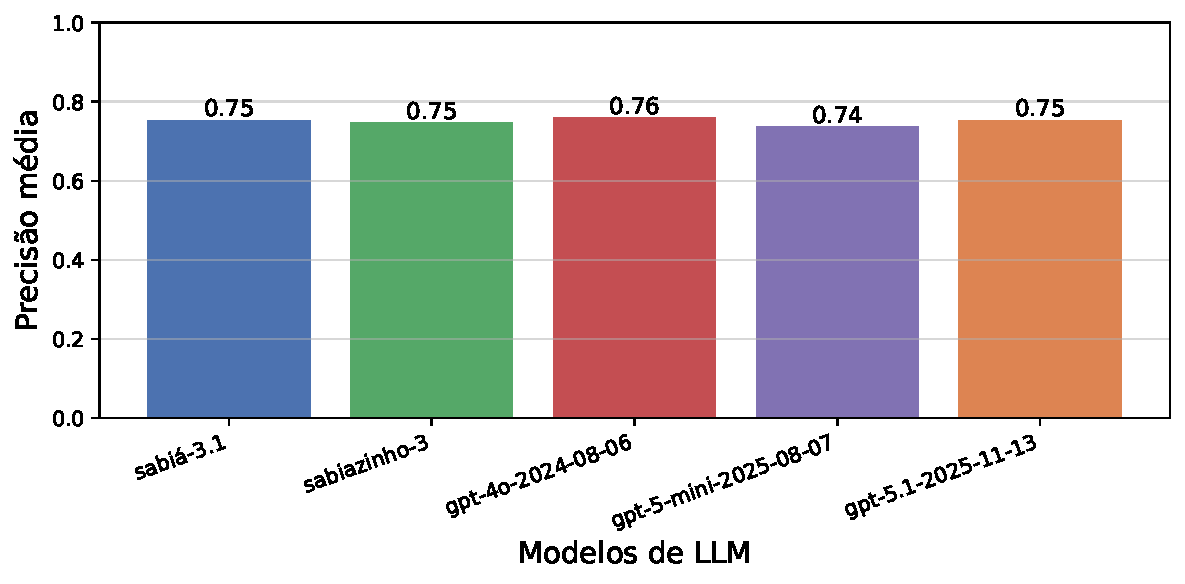
\includegraphics[width=\linewidth]{precisao_media.pdf}
        \caption{Precisão média dos modelos de LLM.}
        \label{fig:precisao-media}
    \end{minipage}
    
    \vspace{0.4cm}
    
    % Segunda linha (1 figura centralizada)
    \begin{minipage}{0.49\textwidth}
        \centering
        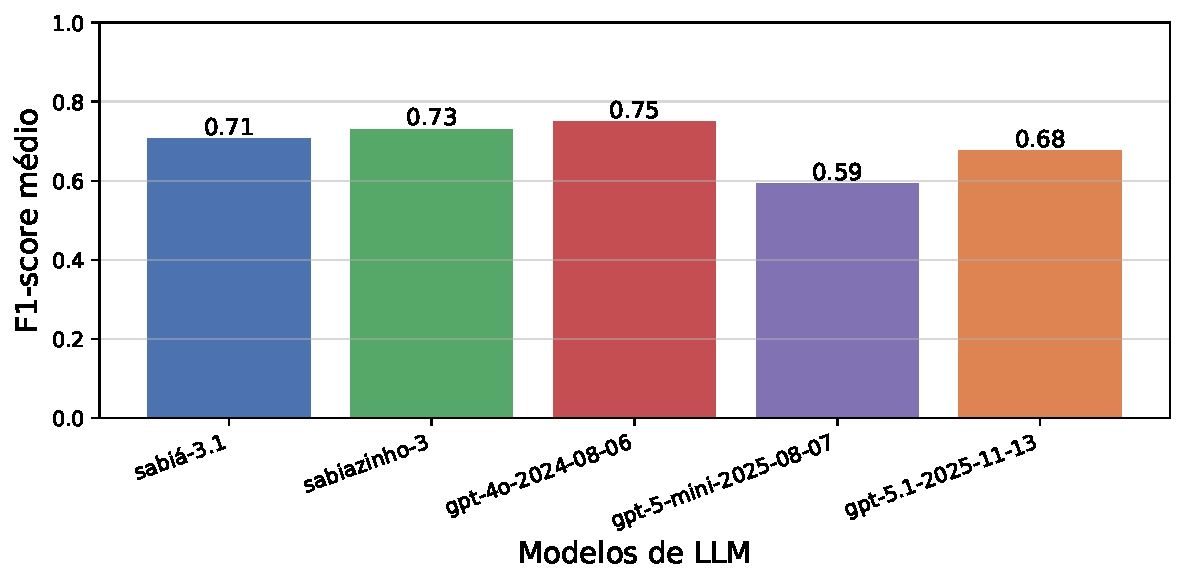
\includegraphics[width=\linewidth]{f1_medio.pdf}
        \caption{F1-score médio dos modelos de LLM.}
        \label{fig:f1-media}
    \end{minipage}
\end{figure}


    
\end{comment}

Ao incorporar o custo à análise, conforme valores apresentados na Tabela~\ref{tab:preco}, observa-se que o desempenho adicional do \textit{GPT-4o} está associado a um custo substancialmente mais elevado por milhão de \textit{tokens}, tanto na entrada quanto na saída. Nesse contexto, o \textit{Sabiazinho 3} destaca-se por apresentar desempenho próximo ao do \textit{GPT-4o}, aliado a um custo significativamente inferior. No caso do \textit{GPT-5-mini}, apesar do menor custo, apresentou desempenho inferior nas métricas avaliadas, com redução mais acentuada na Acurácia de Renda Fixa. Esse resultado sugere que a economia proporcionada por esse modelo tende a ocorrer à custa de menor qualidade na classificação, o que pode limitar sua adequação em cenários que exigem maior robustez analítica.

De forma transversal a todos os modelos, o domínio de Ações apresentou os menores níveis de desempenho, independentemente da métrica considerada. Esse padrão sugere maior ambiguidade semântica e maior dificuldade na delimitação do impacto do conteúdo textual sobre esse tipo de ativo. Adicionalmente, identificaram-se casos em que notícias relacionadas exclusivamente a FIIs foram classificadas como positivas para Ações, enquanto o \textit{dataset} de referência as rotulou como neutras por ausência de impacto direto. Esse comportamento evidencia limitações na distinção entre domínios correlatos e reforça a necessidade de ajustes no \textit{prompt} para explicitar essas fronteiras semânticas.

A análise do tempo de processamento também foi considerada, uma vez que reforça as diferenças operacionais entre os modelos. O \textit{GPT-5-mini} apresentou o maior tempo total de execução, com aproximadamente 253 minutos para classificar 1.884 textos. Em contrapartida, o \textit{Sabiazinho 3} demonstrou maior eficiência, pois concluiu a mesma tarefa em 32 minutos e 52 segundos, conforme ilustrado na Figura~\ref{fig:tempo-total}. 

%\textcolor{red}{Figura 8 é melhor estar para cima}

\begin{comment}
\begin{figure}[h!]
    \centering
        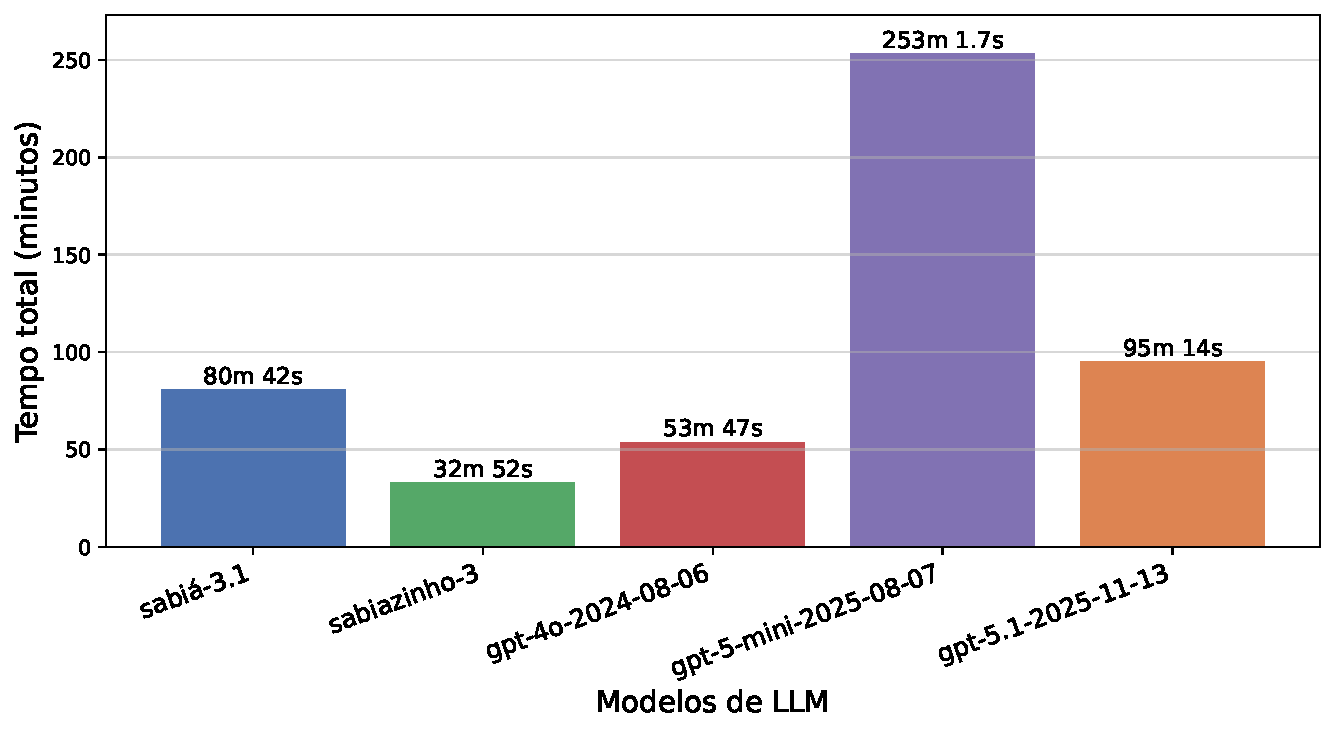
\includegraphics[width=0.5\linewidth]{tempo_total_para_1884.pdf}
        \caption{Tempo total de 1884 classificações por LLM.}
        \label{fig:tempo-total}
\end{figure}
\end{comment}

O GPT-5-mini registrou a maior média, com 8.06 segundos por notícia, enquanto o \textit{Sabiazinho-3} foi o mais eficiente, com apenas 1,05 segundos por item, conforme mostra a Figura \ref{fig:tempo-por-seg}.

%\textcolor{red}{Figura 8 é melhor estar para cima}
\begin{comment}
\begin{figure}[h!]
    \centering
        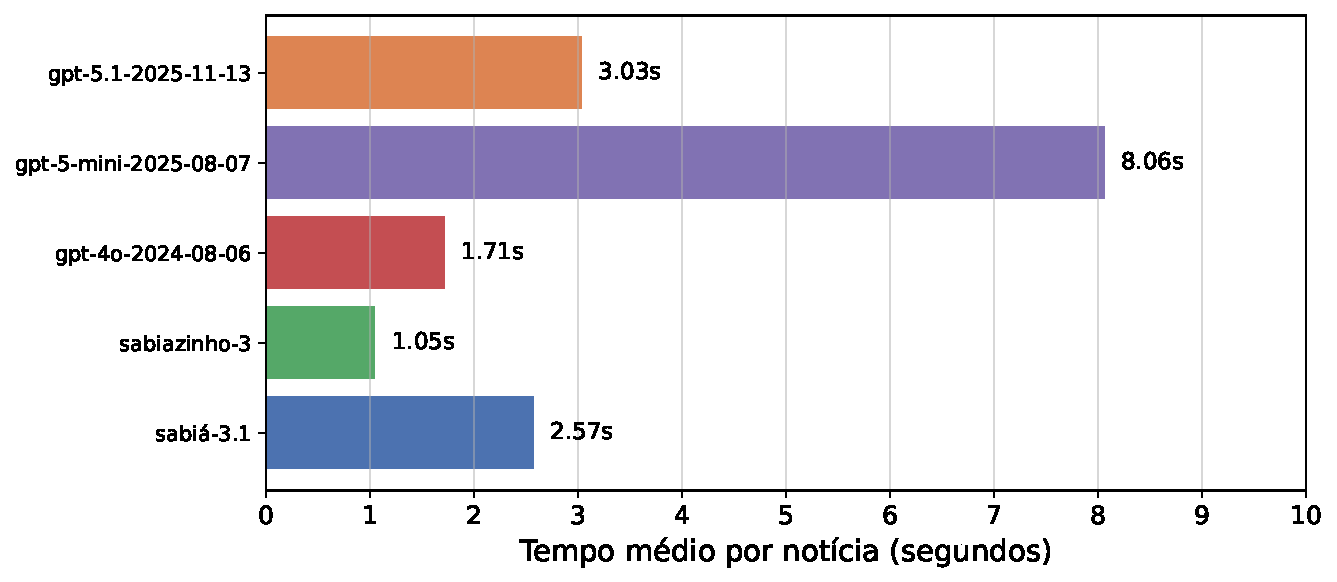
\includegraphics[width=0.5\linewidth]{tempo_medio_por_noticia.pdf}
        \caption{Tempo médio de processamento por notícia.}
        \label{fig:tempo-por-seg}
\end{figure}
\end{comment}

\begin{figure}[h!]
    \centering

    \begin{minipage}{0.48\linewidth}
        \centering
        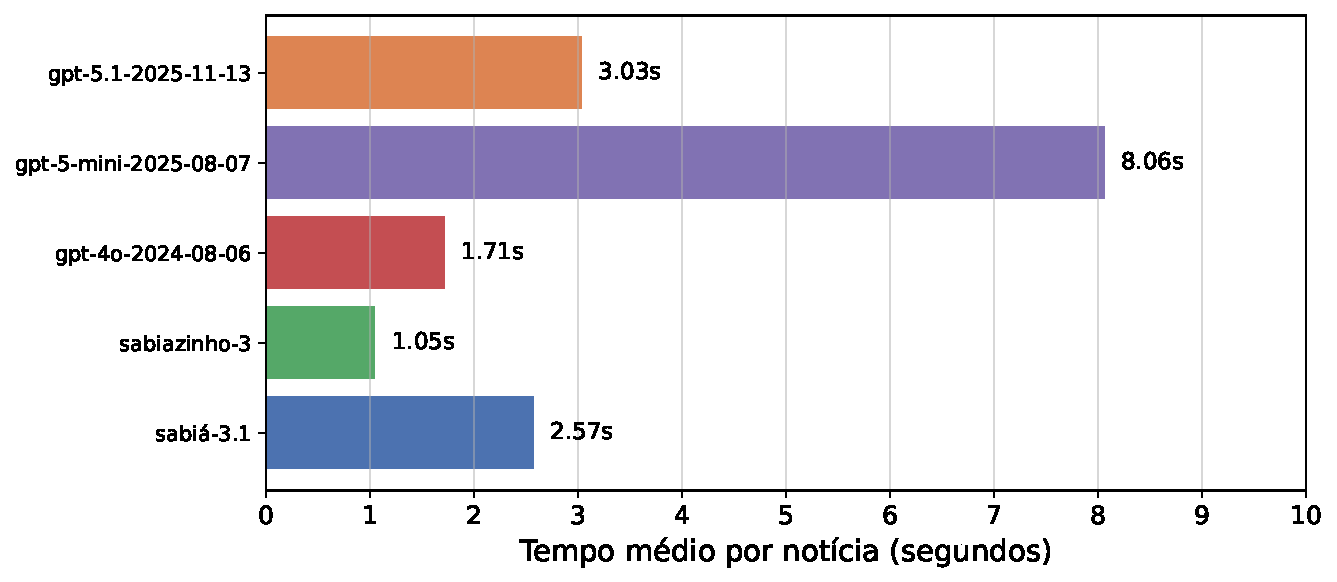
\includegraphics[width=\linewidth]{tempo_medio_por_noticia.pdf}
        \caption{Tempo médio de processamento por notícia.}
        \label{fig:tempo-total}
    \end{minipage}
    \hfill
    \begin{minipage}{0.48\linewidth}
        \centering
        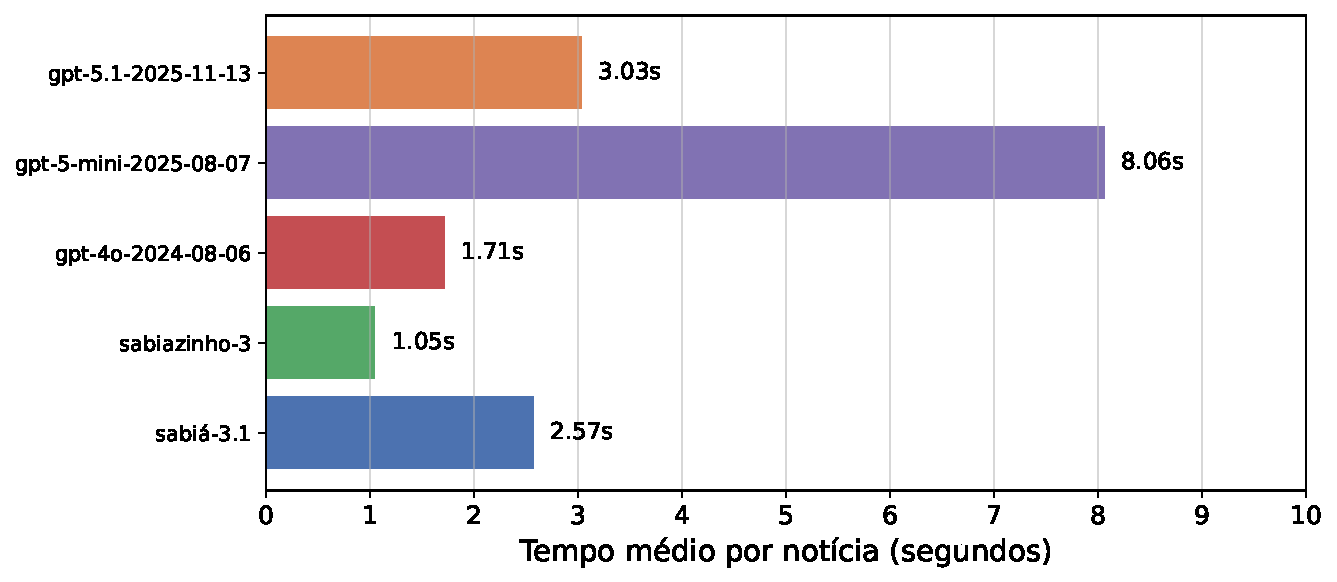
\includegraphics[width=\linewidth]{tempo_medio_por_noticia.pdf}
        \caption{Tempo médio de processamento por notícia.}
        \label{fig:tempo-por-seg}
    \end{minipage}

\end{figure}

Esse comportamento pode ser explicado pelo fato de o GPT-5-mini e o GPT-5.1 pertencerem à classe de \textit{reasoning models}, os quais executam etapas adicionais de raciocínio antes de gerar a resposta. Esse processamento extra introduz um custo computacional fixo por requisição e aumenta o tempo de execução em cenários com chamadas síncronas. Por outro lado, o Sabiá 3.1, o Sabiazinho-3 e o GPT-4o não utilizam mecanismos explícitos de raciocínio, o que contribui para seus menores tempos de processamento.

\begin{comment}
\begin{figure}[h!]
    \centering
    \begin{minipage}{0.49\textwidth}
        \centering
        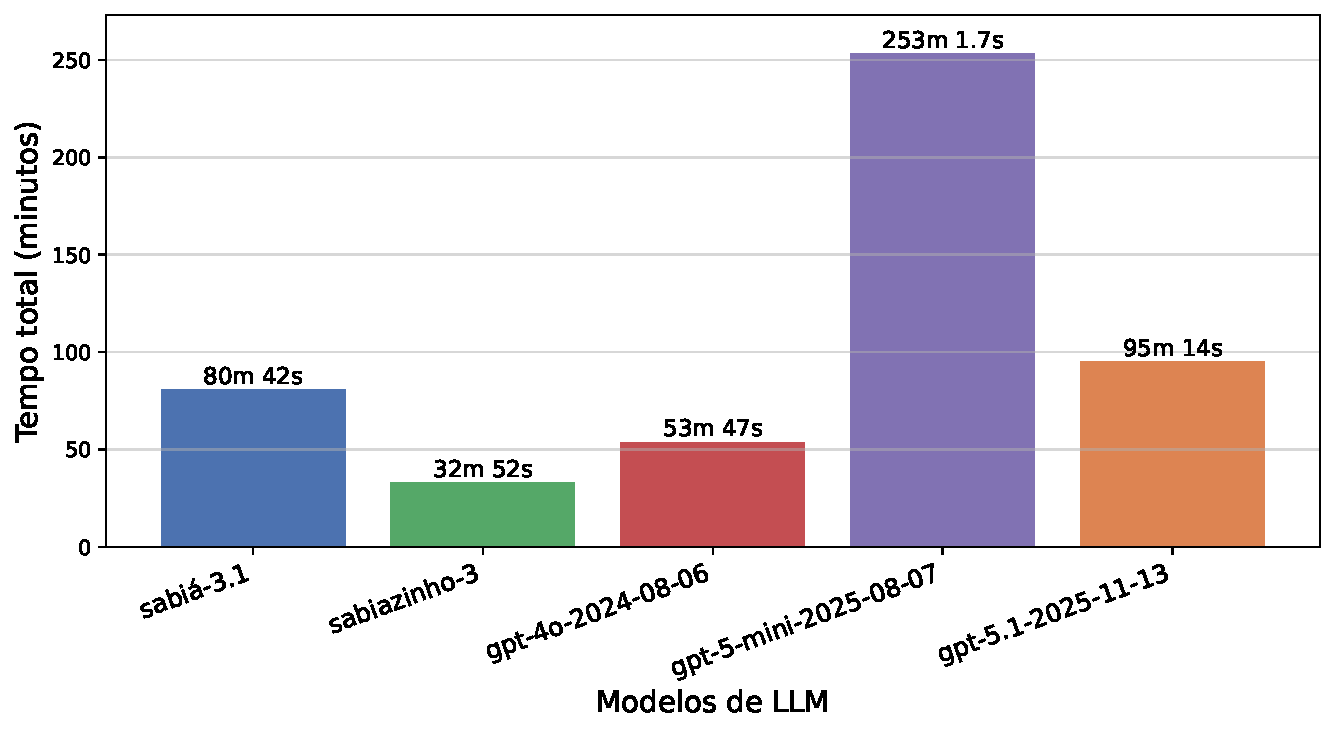
\includegraphics[width=\linewidth]{tempo_total_para_1884.pdf}
        \caption{Tempo total de 1884 classificações por LLM.}
        \label{fig:tempo-total}
    \end{minipage}
    \hfill
    \begin{minipage}{0.49\textwidth}
        \centering
        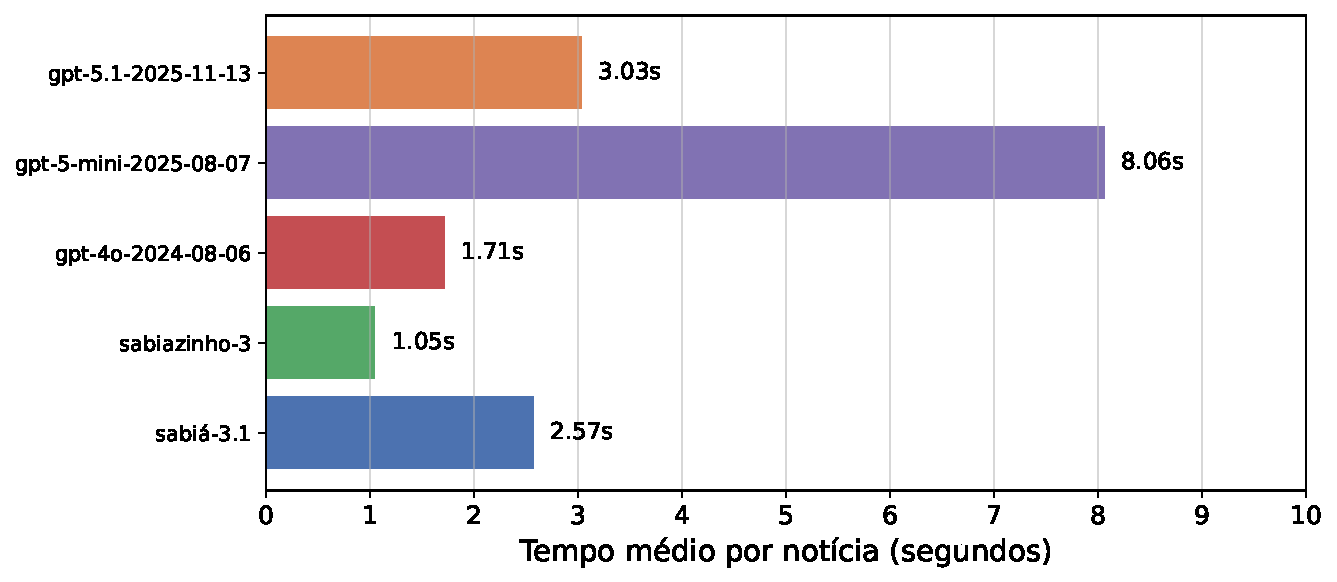
\includegraphics[width=\linewidth]{tempo_medio_por_noticia.pdf}
        \caption{Tempo médio de processamento por notícia.}
        \label{fig:tempo-por-seg}
    \end{minipage}
\end{figure}
\end{comment}

Diante dos resultados obtidos, optou-se pela adoção do \textit{Sabiazinho 3} como modelo principal da \textit{AraraFin}, pois apresentou desempenho competitivo em relação aos modelos da família \textit{GPT}, aliado a um custo significativamente inferior. Conforme a Tabela~\ref{tab:preco}, seu custo por milhão de tokens é aproximadamente 14 vezes menor na entrada e 18 vezes menor na saída quando comparado ao \textit{GPT-4o}. Essa diferença, associada ao menor tempo de processamento observado, torna o \textit{Sabiazinho 3} a alternativa mais eficiente sob a perspectiva de custo-benefício, sem prejuízo relevante à qualidade da classificação.


\subsection{Análise Comparativa com \textit{FinBERT-PT-BR}}

%Após a definição do LLM principal da \textit{AraraFin}, foi conduzido um estudo comparativo com a ferramenta mais difundida na área (i.e., \textit{FinBERT-PT-BR} \cite{santos2023finbert}). Esse modelo, pioneiro em sua proposta, realiza a Análise de Sentimentos em textos relacionados ao mercado financeiro brasileiro e representou um marco relevante para a área. Diante disso, tornou-se pertinente estabelecer uma comparação entre esse modelo consolidado e a aplicação proposta neste trabalho.

Após a definição do LLM principal da \textit{AraraFin}, foi conduzido um estudo comparativo com a ferramenta mais difundida na área (i.e., \textit{FinBERT-PT-BR} \cite{santos2023finbert}). A avaliação foi realizada com o mesmo \textit{dataset} e no mesmo ambiente computacional descritos na Seção~\ref{subsec:pipeline-experimental}. Ou seja, o FinBERT-PT-BR recebeu como entrada os resumos dos textos originais. Diferentemente dos modelos baseados em API, o \textit{FinBERT-PT-BR} foi executado localmente, por se tratar de um modelo disponibilizado pela biblioteca \textit{Hugging Face}, o que elimina custos e latências associadas a requisições externas. Nessas condições, o modelo levou aproximadamente 18,5 segundos para classificar 628 notícias, o que corresponde a um tempo médio de cerca de 0,03 segundos por instância. Ressalta-se que o \textit{FinBERT-PT-BR} não permite a parametrização explícita do domínio de investimento, pois realiza a classificação de sentimento sob uma perspectiva geral.

Os resultados apresentados na Tabela~\ref{tab:gpt-fin} indicam que \textit{AraraFin} superou o \textit{FinBERT-PT-BR} em todas as métricas. Destaca-se, em especial, o desempenho em FIIs e Renda Fixa, nos quais a \textit{AraraFin} alcançou valores de acurácia duas ou mais vezes superiores. Na categoria de Ações, também foram observados ganhos consistentes, com aumento em torno de 12\% na acurácia. Esses resultados indicam que a abordagem baseada em \textit{LLMs} com \textit{prompts} especializados por domínio é mais eficaz para capturar nuances semânticas específicas do mercado financeiro do que modelos treinados de forma genérica. Apesar disso, o Ararafin ainda não atingiu um valor adequado para o domínio de investimentos de Ações, o que geralmente é mais volátil, mas se mostrou bem adequado para os domínios de Fundos de Investimentos Imobiliários e Renda Fixa.

\begin{comment}
\begin{table}[h!]
\centering
\caption{Comparação de desempenho entre \textit{AraraFin} e \textit{FinBERT-PT-BR}.}
\label{tab:gpt-fin}
\begin{tabular}{|l|l|c|c|}
\hline
\textbf{Categoria} & \textbf{Métrica} & \textbf{\textit{AraraFin}} & \textbf{\textit{FinBERT-PT-BR}} \\
\hline
\multirow{3}{*}{FIIs} 
  & Acurácia  & \textbf{0.83} & 0.38 \\
  & Precisão  & \textbf{0.82} & 0.62 \\
  & \textit{F1-score}  & \textbf{0.81} & 0.36 \\
\hline
\multirow{3}{*}{Renda Fixa} 
  & Acurácia  & \textbf{0.83} & 0.17 \\
  & Precisão  & \textbf{0.84} & 0.82 \\
  & \textit{F1-score} & \textbf{0.84} & 0.25 \\
\hline
\multirow{3}{*}{Ações} 
  & Acurácia  & \textbf{0.55} & 0.49 \\
  & Precisão  & \textbf{0.58} & 0.54 \\
  & \textit{F1-score}  & \textbf{0.54} & 0.45 \\
\hline
\end{tabular}
\end{table}
\end{comment}

\begin{table}[!htb]
\centering
\caption{Comparação de desempenho entre \textit{AraraFin} e \textit{FinBERT-PT-BR}.}
\label{tab:gpt-fin}
\resizebox{0.4\textwidth}{!}{%
\begin{tabular}{@{}llcc@{}}
\toprule
\textbf{Categoria} & \textbf{Métrica} & \textbf{\textit{AraraFin}} & \textbf{\textit{FinBERT-PT-BR}} \\
\midrule

\multirow{3}{*}{FIIs} 
 & Acurácia  & \textbf{0.83} & 0.38 \\
 & Precisão  & \textbf{0.82} & 0.62 \\
 & \textit{F1-score}  & \textbf{0.81} & 0.36 \\
\midrule

\multirow{3}{*}{Renda Fixa} 
 & Acurácia  & \textbf{0.83} & 0.17 \\
 & Precisão  & \textbf{0.84} & 0.82 \\
 & \textit{F1-score} & \textbf{0.84} & 0.25 \\
\midrule

\multirow{3}{*}{Ações} 
 & Acurácia  & \textbf{0.55} & 0.49 \\
 & Precisão  & \textbf{0.58} & 0.54 \\
 & \textit{F1-score}  & \textbf{0.54} & 0.45 \\
\bottomrule

\end{tabular}%
}
\end{table}

%Durante os testes com o \textit{FinBERT-PT-BR}, observou-se uma tendência dele classificar como positivas, notícias que continham termos como “aumentou” ou “cresceu”, independentemente do contexto. Tal comportamento resultou em interpretações equivocadas, especialmente no caso de FIIs: por exemplo, ``aumento da vacância de um imóvel'', embora seja uma notícia negativa para o contexto de FIIs, foi classificado erroneamente como positivo. Apesar disso, o Ararafin ainda não atingiu um valor adequado para o domínio de investimentos de Ações, o que geralmente é mais volátil, mas se mostrou bem adequado para os domínios de Fundos de Investimentos Imobiliários e Renda Fixa. %O mesmo se aplicou a notícias sobre o aumento da taxa SELIC, que foram interpretadas como positivas, mesmo que o impacto dependa do tipo de ativo analisado.



%Esses resultados evidenciam que a abordagem generalista do \textit{FinBERT-PT-BR} é insuficiente para capturar as nuances semânticas específicas de cada domínio de investimento, o que reforça a relevância da segmentação adotada pela \textit{AraraFin}.


\section{Conclusão}

Este trabalho apresentou a \textit{AraraFin}, uma solução baseada em LLMs para análise de sentimentos no mercado financeiro brasileiro, com classificação sensível ao domínio de investimento. Os resultados demonstraram desempenho superior ao de \textit{FinBERT-PT-BR} em todas as modalidades, com ganhos de acurácia superiores a 
100\% em FIIs e Renda Fixa, e de aproximadamente 12\% em Ações. A abordagem baseada em \textit{prompt engineering} com segmentação por domínio mostrou-se uma alternativa 
viável e economicamente eficiente em relação ao \textit{fine-tuning}, ao eliminar a necessidade de grandes conjuntos de dados rotulados e viabilizar a incorporação de conhecimento de domínio diretamente nas instruções fornecidas ao modelo.

A ferramenta contribui para preencher uma lacuna identificada na literatura, marcada pela escassez de soluções voltadas à Análise de Sentimentos em textos financeiros escritos em português: um domínio dinâmico e repleto de nuances específicas. Além disso, a \textit{AraraFin} oferece maior transparência nas classificações em relação a ferramentas frequentemente descritas como “caixas-pretas” \cite{jim2024recent}, pois evidencia as justificativas de cada classificação e promove uma maior confiabilidade. Este trabalho
disponibiliza ainda, como contribuição à comunidade, o \textit{dataset} com 628 notícias financeiras classificadas por domínio de investimento, com o objetivo de fomentar pesquisas futuras neste campo.

De modo geral, os resultados obtidos foram satisfatórios (para os domínios de FIIs e Renda Fixa), especialmente pela capacidade da solução de lidar com eventos cuja carga semântica varia conforme 
o contexto, o que evidencia limitações presentes em modelos como o \textit{FinBERT-PT-BR}. Os resultados do domínio de Ações precisam ser refinados em atualizações futuras do \textit{Ararafin}.
O refinamento das diretrizes de anotação para o domínio de Renda Fixa também é importante, com vistas a elevar a concordância entre avaliadores nesse domínio. Ainda assim, mesmo com concordância razoável ($\kappa = 0{,}35$), a \textit{AraraFin} superou o \textit{FinBERT-PT-BR} em mais de 100\% nesse domínio, resultado expressivo dado que, por sua natureza, Renda Fixa é o segmento de menor volatilidade e impacto entre os analisados.
Além disso, pretende-se aprimorar os \textit{prompts} utilizados para incluir dados históricos e indicadores macroeconômicos atualizados dinamicamente, além de dados multimodais, tais como áudios, vídeos e imagens, que ampliem a cobertura analítica. Por fim, a \textit{AraraFin} deve ser utilizada como uma ferramenta complementar, para suporte à análise e à previsão de movimentos do mercado financeiro, com o objetivo de promover decisões mais embasadas e seguras.




\bibliographystyle{sbc}
\bibliography{sbc-template}

\end{document}
